% !TEX encoding = UTF-8
% !TEX program = pdflatex
% !TEX root = presentazione.tex
% !TeX spellcheck = it_IT

%----------------------------------------------------------------------------------------
%	PACKAGES AND MISC SETTINGS
%----------------------------------------------------------------------------------------

\documentclass[12pt]{beamer}
%\documentclass[12pt,aspectratio=169]{beamer}
%\documentclass[12pt,aspectratio=43]{beamer}
\usepackage[italian]{babel}
\usepackage[utf8]{inputenc}
\usepackage{tabularx}
\usepackage{booktabs}
\usepackage{graphicx}
\usetheme[pageofpages=di,% String used between the current page and the
                         % total page count.
          bullet=circle,% Use circles instead of squares for bullets.
          titleline=true,% Show a line below the frame title.
          alternativetitlepage=true,% Use the fancy title page.
          titlepagelogo=unipd-pollo,% Logo for the first page.
          watermark=logo-unipd-int% Watermark used in every page.
          ]{Torino}

\hypersetup{
	pdftitle={Servizi cognitivi e analisi visiva},
	pdfauthor={Marco Romanelli},
	pdfstartview={Fit},
	pdfstartpage=1,
	bookmarks=true,
	bookmarkstype=toc,
	bookmarksopen=true,
	pdfhighlight=/I,
	pdfpagemode=FullScreen
}
\usepackage{alltt}
\usepackage{tikz}
\usepackage{graphicx}
\usepackage{appendixnumberbeamer}
\usepackage{cclicenses}

\newcolumntype{?}{!{\vrule width 0.3mm}}

\graphicspath{{../img/}}

%----------------------------------------------------------------------------------------
%	TITLE PAGE
%----------------------------------------------------------------------------------------

\author[Romanelli,Marco]{Marco Romanelli\\[0.5\baselineskip]
\tiny marco.romanelli.1@studenti.unipd.it\\[1.5\baselineskip]
\scriptsize Corso di Intelligenza Artificiale}

\title{Servizi cognitivi e analisi visiva}
\course{Laurea Magistrale in Informatica}
\institute{Universit\`a di Padova}
\date{4 luglio 2017}

\begin{document}

\section{Introduzione}\label{sec:intro}
\begin{frame}[t,plain]\titlepage\end{frame}

	%----------------------------------------------------------------------------------------
	%	BODY
	%----------------------------------------------------------------------------------------

	\setcounter{framenumber}{0} % start from here
	% !TEX encoding = UTF-8
% !TEX program = pdflatex
% !TEX root = presentazione.tex
% !TeX spellcheck = it_IT

%----------------------------------------------------------------------------------------
%	APPUNTI GENERALI:
% 		-
%		-
%----------------------------------------------------------------------------------------


%----------------------------------------------------------------------------------------
%	CONTENUTO PRINCIPALE
%----------------------------------------------------------------------------------------
\section{Contenuto}\label{sec:contenuto}


	%----------------------------------------------------------------------------------------
	%	SERVIZI COGNITIVI
 	%----------------------------------------------------------------------------------------
	% !TEX encoding = UTF-8
% !TEX program = pdflatex
% !TEX root = presentazione.tex
% !TeX spellcheck = it_IT
%
\begin{frame}[t]{Servizi cognitivi}
\begin{itemize}
	\item Creare applicazioni in grado di analizzare e interpretare la realtà
	\item Aree principali:
	\begin{itemize}
		\item Visione
		\item Linguaggio
		\item Ricerca
		\item Conoscenza
	\end{itemize}
\end{itemize}
\end{frame}
%
%----------------------------------------------------------------------------------------
%	APPUNTI:
%		- realizzare applicazioni in grado di analizzare e interpretare la realtà
% 		- l’area di visione racchiude quelle tecniche per l’analisi, la rappresentazione di immagini e video
%		- area del lingaggio fornisce strumenti per capire meglio cosa vuole l’utente tramite l’interpretazione
%			della scrittura o del linguaggio naturale.
%----------------------------------------------------------------------------------------


	%----------------------------------------------------------------------------------------
	%	I SERVIZI COGNITIVI - parte 2
	%----------------------------------------------------------------------------------------
	% !TEX encoding = UTF-8
% !TEX program = pdflatex
% !TEX root = presentazione.tex
% !TeX spellcheck = it_IT
%
\begin{frame}[t]{Servizi cognitivi - 2}
\begin{itemize}
	\item Microsoft Cognitive Services (Microsoft Corporation)
	\begin{itemize}
		\item Computer Vision API
		\item Content Moderator API
		\item Face (Emotion) API
	\end{itemize}
	\item Watson Services (Bluemix) (IBM)
	\begin{itemize}
		\item Visual Recognition
	\end{itemize}
	\item Amazon Artificial Intelligence (Amazon.com, Inc)
	\begin{itemize}
		\item Amazon Rekognition
	\end{itemize}
	\item Google Cloud Machine Learning Services (Google Inc.)
	\begin{itemize}
		\item Cloud Vision API
	\end{itemize}
\end{itemize}
\end{frame}
%
%----------------------------------------------------------------------------------------
%	APPUNTI:
% 		- Si vede un punto alla volta, quindi si può partire con una cosa del genere:
%			"... come abbiamo detto ci focalizzeremo nei servizi che ricadono sotto l'area di Visione"
%				e poi legare con
%			"quattro delle maggiori aziende del settore offrono..."
%----------------------------------------------------------------------------------------


	%----------------------------------------------------------------------------------------
	%	MICROSOFT - 0
	%----------------------------------------------------------------------------------------
	% !TEX encoding = UTF-8
% !TEX program = pdflatex
% !TEX root = presentazione.tex
% !TeX spellcheck = it_IT
%
\begin{frame}[t]{Microsoft Cognitive Services}
	\begin{figure}[!h]
	\centering
	\vfill
	
\includegraphics[width=.4\paperwidth,keepaspectratio=true]{loghi/microsoft-cs}
	\vfill
	\end{figure}
\end{frame}
%
%----------------------------------------------------------------------------------------
%	APPUNTI:
%		-
%----------------------------------------------------------------------------------------


	%----------------------------------------------------------------------------------------
	%	MICROSOFT
	%----------------------------------------------------------------------------------------
	% !TEX encoding = UTF-8
% !TEX program = pdflatex
% !TEX root = presentazione.tex
% !TeX spellcheck = it_IT
%
\begin{frame}[t]{Microsoft Computer Vision API}
\begin{itemize}
	\item Riconoscimento elementi dell'immagine
	\item Classificazione
	\item Riconoscimento volti
	\item Riconoscimento del testo
	\item Generazione di descrizioni
	\item Riconoscimento contenuti non adatti ai minori
	\item Altro:
	\begin{itemize}
		\item Creazione anteprime
		\item Identificazione tipo, colori e qualità immagine
		\item Estensione classificatore
	\end{itemize}
\end{itemize}
\end{frame}
%
%----------------------------------------------------------------------------------------
%	APPUNTI:
% 		- elementi come: oggetti, esseri viventi, azioni; oltre 2000
%			-ritorna un insieme di etichette (in formato JSON) che descrivono gli oggetti presenti nell’immagine
%		- classificazione secondo una tassonomia composta da 86 categorie
%		- identifica la posizione del volto e età/sesso
%		- testo presente nell'immagine e testo scritto a mano
%		- frase/i (in inglese) che descrive l'immagine
%		- le varie categorie comprendono gruppi per contenuti e non adatti a minori
%		- Estensione classificatore (Contenuto personalizzato):
%			- servirebbe appunto per estendere la tassonomia predefinita
%			- ad oggi è supportato solo: riconscimento personaggi famosi e oggetti di interesse (landmark)
%----------------------------------------------------------------------------------------


	%----------------------------------------------------------------------------------------
	%	MICROSOFT
	%----------------------------------------------------------------------------------------
	% !TEX encoding = UTF-8
% !TEX program = pdflatex
% !TEX root = presentazione.tex
% !TeX spellcheck = it_IT
%
\begin{frame}[t]{Microsoft Computer Vision API - Esempio}
	\begin{figure}[h]
	\centering
	    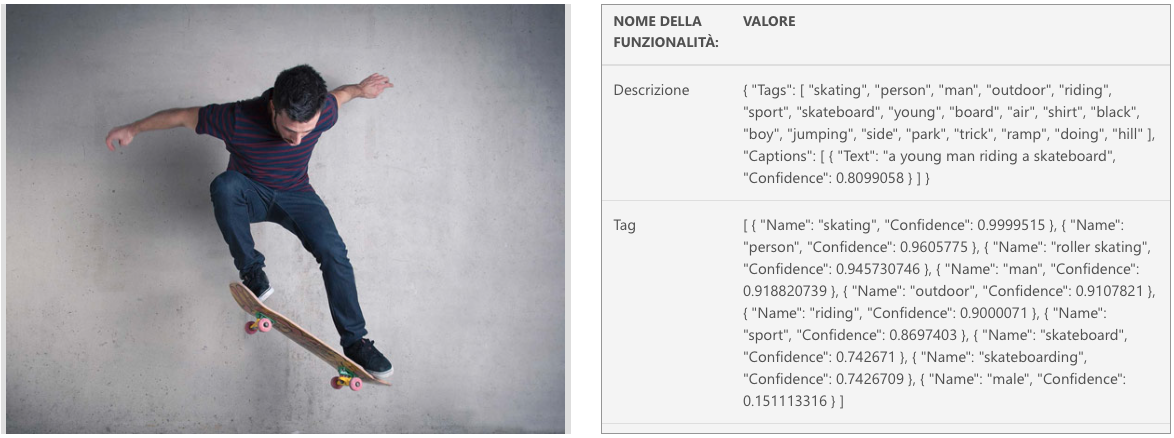
\includegraphics[width=\textwidth,keepaspectratio=true]{esempio-microsoft}
		\label{fig:esempio-microsoft}
	\end{figure}
\end{frame}
%
%----------------------------------------------------------------------------------------
%	APPUNTI:
% 		-
%----------------------------------------------------------------------------------------


	%----------------------------------------------------------------------------------------
	%	MICROSOFT - 5
	%----------------------------------------------------------------------------------------
	% !TEX encoding = UTF-8
% !TEX program = pdflatex
% !TEX root = presentazione.tex
% !TeX spellcheck = it_IT
%
\begin{frame}[t]{Microsoft Computer Vision API - Esempio (2)}
	\begin{figure}[h]
	\centering
	    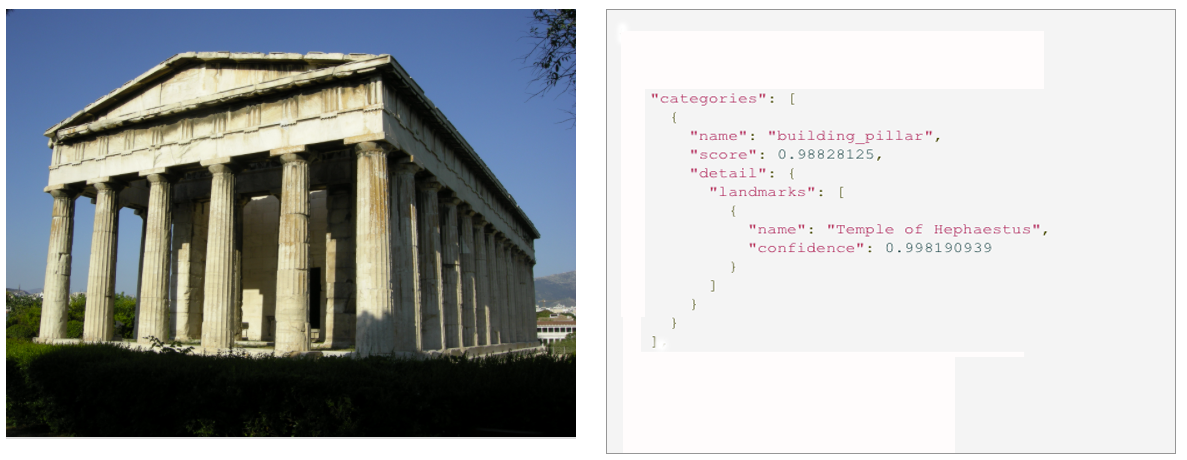
\includegraphics[width=\textwidth,keepaspectratio=true]{esempi-microsoft/landmark}
		\label{fig:esempio-microsoft-2}
	\end{figure}
\end{frame}
%
%----------------------------------------------------------------------------------------
%	APPUNTI:
% 		- Tempo di Efesto
%----------------------------------------------------------------------------------------


	%----------------------------------------------------------------------------------------
	%	MICROSOFT - 2
	%----------------------------------------------------------------------------------------
	% !TEX encoding = UTF-8
% !TEX program = pdflatex
% !TEX root = presentazione.tex
% !TeX spellcheck = it_IT
%
\begin{frame}[t]{Microsoft Content Moderator API}
\begin{itemize}
	\item Tre tipi di operazioni:
	\begin{itemize}
		\item Rilevare la presenza di pornografici e osé in generale
		\item Rilevare la presenza di volti di persone
		\item Contenuti personalizzati
		\begin{itemize}
			\item Confronto fra immagini
			\item Identificazione contenuto: alcool, nudità, armi, violenza, volgarità, eccetera
		\end{itemize}
	\end{itemize}
\end{itemize}
\end{frame}
%
%----------------------------------------------------------------------------------------
%	APPUNTI:
%		- Evaluate: come sopra
% 		- Find faces: potrebbe essere utilizzato, ad esempio, per evitare che gli utenti inviino informazioni personali
%		- Match: possibile creare e personalizzare una lista dei contenuti che si vogliono bloccare
%			- confronta le immagini caricate con quelle presenti nella lista
%			-  i doppioni ma anche versioni leggermente modificate
%			- Nudity Sexual Content, alcohol Tobacco Drugs Child Exploitation Violence Weapons Gore Profanity Vulgarity
%----------------------------------------------------------------------------------------


	%----------------------------------------------------------------------------------------
	%	MICROSOFT - 3
	%----------------------------------------------------------------------------------------
	% !TEX encoding = UTF-8
% !TEX program = pdflatex
% !TEX root = presentazione.tex
% !TeX spellcheck = it_IT
%
\begin{frame}[t]{Microsoft Face API e Emotion API}
\begin{itemize}
	\item Rilevamento volti
	\item Confronto fra due volti
	\item Confronto/ricerca in un insieme di volti
	\item Emozioni: rabbia, paura, felicità, espressione neutra, tristezza, sorpresa, disprezzo e disgusto
\end{itemize}
\end{frame}
%
%----------------------------------------------------------------------------------------
%	APPUNTI:
% 		- più approfondita dei volti rispetto alle Computer Vision API
%			includendo anche funzioni di confronto e ricerca.
%		- Rileva i volti presenti nell’immagine (fino a 64) e restituisce le coordinate
%			del rettangolo che ingloba il viso, gli attributi facciali e i punti di riferimento.
%		- attributi facciali: eta, sesso, sorriso, tipologia di barba, la posizione tridimensionale
%			del volto (imbardata, rollio e beccheggio), la presenza di occhiali, le emozioni
%			emozioni: rabbia, paura, felicità, espressione neutra, tristezza, sorpresa, disprezzo e disgusto
%		- verifica volto: probabilità che due volti appartengano alla stessa persona
%		- identicificazione volti: identificare le persone sulla base di un volto e di un database di persone
%		- Ricerca volti simili: fornendo un volto obbiettivo e un insieme di candidati  all’interno del quale
%			eseguire la ricerca, questa funzione restituisce un piccolo insieme di volti che assomiglia al volto obiettivo.
%----------------------------------------------------------------------------------------


	%----------------------------------------------------------------------------------------
	%	MICROSOFT -
	%----------------------------------------------------------------------------------------
	% !TEX encoding = UTF-8
% !TEX program = pdflatex
% !TEX root = presentazione.tex
% !TeX spellcheck = it_IT
%
\begin{frame}[t]{Microsoft Computer Face API - Esempio}
	\begin{figure}[h]
	\centering
	    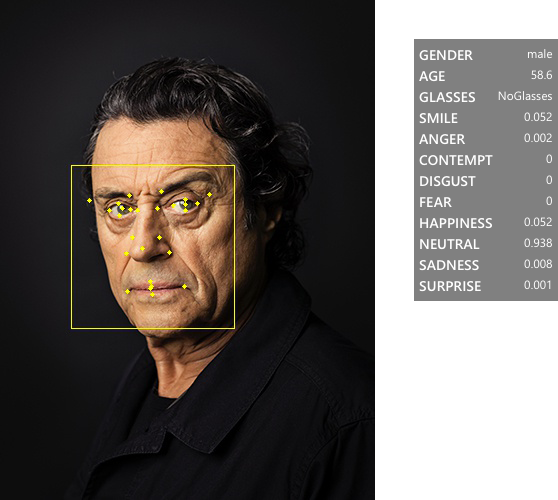
\includegraphics[width=.6\paperwidth,keepaspectratio=true]{esempi-microsoft/face-1}
		\label{fig:esempio-microsoft-face}
	\end{figure}
\end{frame}
%
%----------------------------------------------------------------------------------------
%	APPUNTI:
% 		-
%----------------------------------------------------------------------------------------


	%----------------------------------------------------------------------------------------
	%	IBM - 0
	%----------------------------------------------------------------------------------------
	% !TEX encoding = UTF-8
% !TEX program = pdflatex
% !TEX root = presentazione.tex
% !TeX spellcheck = it_IT
%
\begin{frame}[t]{IBM Watson Services (Bluemix)}
	\begin{figure}[!h]
	\centering
	\vfill
	
\includegraphics[width=.4\paperwidth,keepaspectratio=true]{loghi/ibm-bluemix}
	\vfill
	\end{figure}
\end{frame}
%
%----------------------------------------------------------------------------------------
%	APPUNTI:
%		-
%----------------------------------------------------------------------------------------


	%----------------------------------------------------------------------------------------
	%	IBM
	%----------------------------------------------------------------------------------------
	% !TEX encoding = UTF-8
% !TEX program = pdflatex
% !TEX root = presentazione.tex
% !TeX spellcheck = it_IT
%
\begin{frame}[t]{IBM Visual Recognition}
\begin{itemize}
	\item Riconscimento elementi (classificazione in categorie)
	\item Riconoscimento volti
	\item Gestione classificatore:
	\begin{itemize}
		\item Creazione
		\item Aggiornamento
		\item Ricerca
	\end{itemize}
\end{itemize}
\end{frame}
%
%----------------------------------------------------------------------------------------
%	APPUNTI:
% 		- viene fornito in riposa una lista di coppie classe-punteggio per ogni classificatore selezionato
%		- Le classi sono organizzate in categorie e sotto-categorie dove il livello piu` astratto
%		comprende categorie quali animali, persone, cibo, sport, natura, eccetera.
%			- l’inglese, spagnolo, arabo o giapponese.
%		- età, sesso o nome del personaggio famoso
%		- immagini insieme positivo e negativo
%		- ricerca tramite Similarity Search
%----------------------------------------------------------------------------------------


	%----------------------------------------------------------------------------------------
	%	IBM - 2
	%----------------------------------------------------------------------------------------
	% !TEX encoding = UTF-8
% !TEX program = pdflatex
% !TEX root = presentazione.tex
% !TeX spellcheck = it_IT
%
\begin{frame}[t]{IBM Visual Recognition - Esempio}
	\begin{figure}[h]
	\centering
	    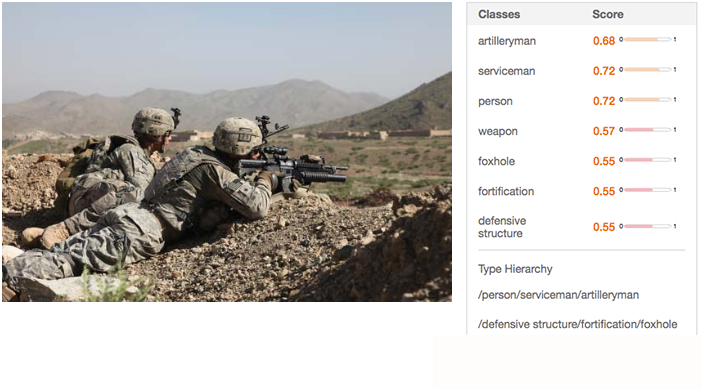
\includegraphics[width=.9\textwidth,keepaspectratio=true]{esempio-ibm}
		\label{fig:esempio-ibm}
	\end{figure}
\end{frame}
%
%----------------------------------------------------------------------------------------
%	APPUNTI:
% 		-
%----------------------------------------------------------------------------------------


	%----------------------------------------------------------------------------------------
	%	AMAZON - 0
	%----------------------------------------------------------------------------------------
	% !TEX encoding = UTF-8
% !TEX program = pdflatex
% !TEX root = presentazione.tex
% !TeX spellcheck = it_IT
%
\begin{frame}[t]{Amazon Artificial Intelligence}
	\begin{figure}[!h]
	\centering
	\vfill
	
\includegraphics[width=.3\paperwidth,keepaspectratio=true]{loghi/amazon-ws}
	\vfill
	\end{figure}
\end{frame}
%
%----------------------------------------------------------------------------------------
%	APPUNTI:
%		-
%----------------------------------------------------------------------------------------


	%----------------------------------------------------------------------------------------
	%	AMAZON
	%----------------------------------------------------------------------------------------
	% !TEX encoding = UTF-8
% !TEX program = pdflatex
% !TEX root = presentazione.tex
% !TeX spellcheck = it_IT
%
\begin{frame}[t]{Amazon Rekognition}
\begin{itemize}
	\item Rilevamento scene e oggetti
	\item Operazioni su volti di persone:
	\begin{itemize}
		\item analisi
		\item confronto
		\item ricerca (collezione personalizzata)
	\end{itemize}
\end{itemize}
\end{frame}
%
%----------------------------------------------------------------------------------------
%	APPUNTI:
% 		- Permette di rilevare automaticamente oggetti e con il relativo punteggio
%			- veicoli, alberi, animali
%			- scene (una spiaggia o un tramonto)
%			- eventi (matrimoni, feste di compleanno)
%			- concetti astratti (serata, paesaggio, natura)
%		- solito: età, sesso, emozioni, punti del viso, sorriso, occhi aperti, baffi, occhiali
%		- confronto: probabilità che due volti appartengano alla stessa persona
%		- ricerca: all'interno di una collezione
%----------------------------------------------------------------------------------------


	%----------------------------------------------------------------------------------------
	%	AMAZON - 2
	%----------------------------------------------------------------------------------------
	% !TEX encoding = UTF-8
% !TEX program = pdflatex
% !TEX root = presentazione.tex
% !TeX spellcheck = it_IT
%
\begin{frame}[t]{Amazon Rekognition - Esempio}
	\begin{figure}[h]
	\centering
	    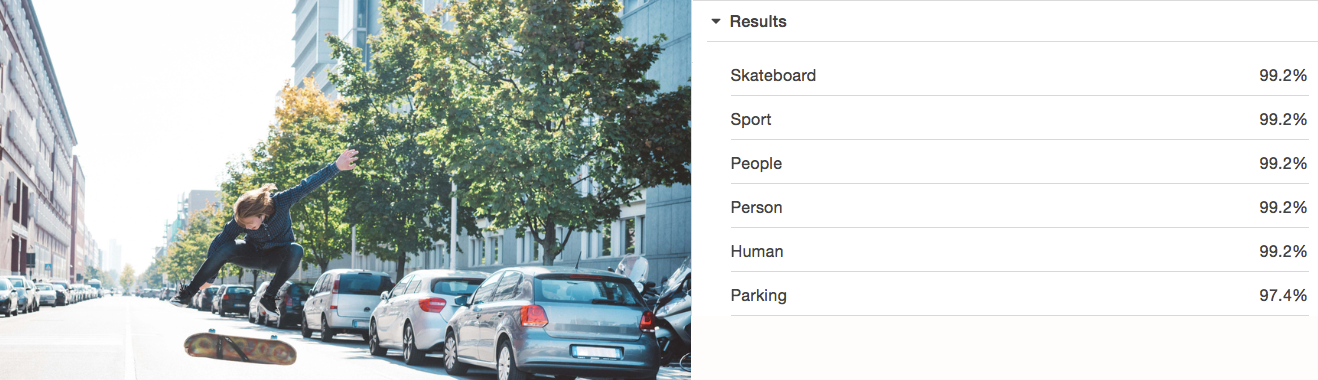
\includegraphics[width=\textwidth,keepaspectratio=true]{esempio-amazon}
		\label{fig:esempio-amazon}
	\end{figure}
\end{frame}
%
%----------------------------------------------------------------------------------------
%	APPUNTI:
% 		-
%----------------------------------------------------------------------------------------


	%----------------------------------------------------------------------------------------
	%	AMAZON - 3
	%----------------------------------------------------------------------------------------
	% !TEX encoding = UTF-8
% !TEX program = pdflatex
% !TEX root = presentazione.tex
% !TeX spellcheck = it_IT
%
\begin{frame}[t]{Amazon Rekognition - Esempio (2)}
	\begin{figure}[h]
	\centering
	    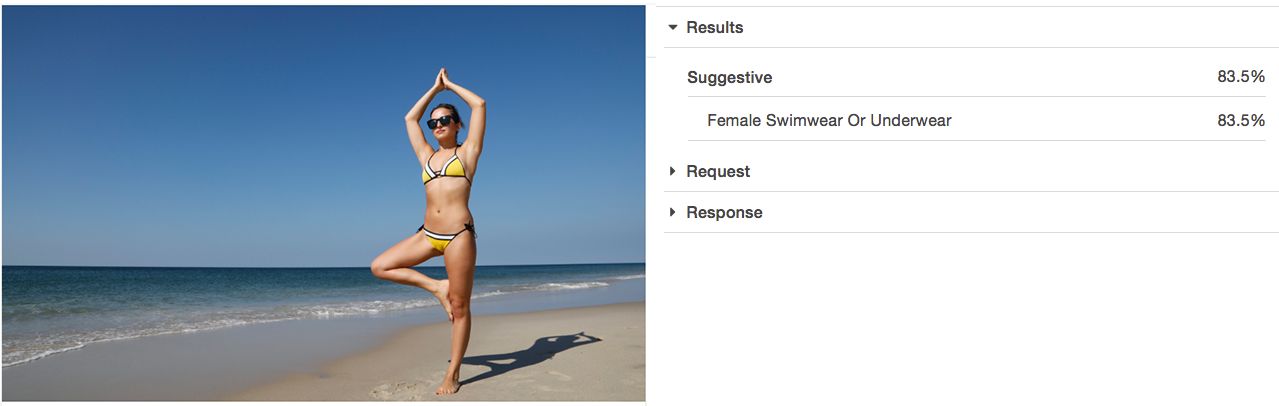
\includegraphics[width=\textwidth,keepaspectratio=true]{esempi-amazon/moderator}
		\label{fig:esempio-amazon}
	\end{figure}
\end{frame}
%
%----------------------------------------------------------------------------------------
%	APPUNTI:
% 		-
%----------------------------------------------------------------------------------------


	%----------------------------------------------------------------------------------------
	%	AMAZON - 4
	%----------------------------------------------------------------------------------------
	% !TEX encoding = UTF-8
% !TEX program = pdflatex
% !TEX root = presentazione.tex
% !TeX spellcheck = it_IT
%
\begin{frame}[t]{Amazon Rekognition - Esempio (3)}
	\begin{figure}[h]
	\centering
	    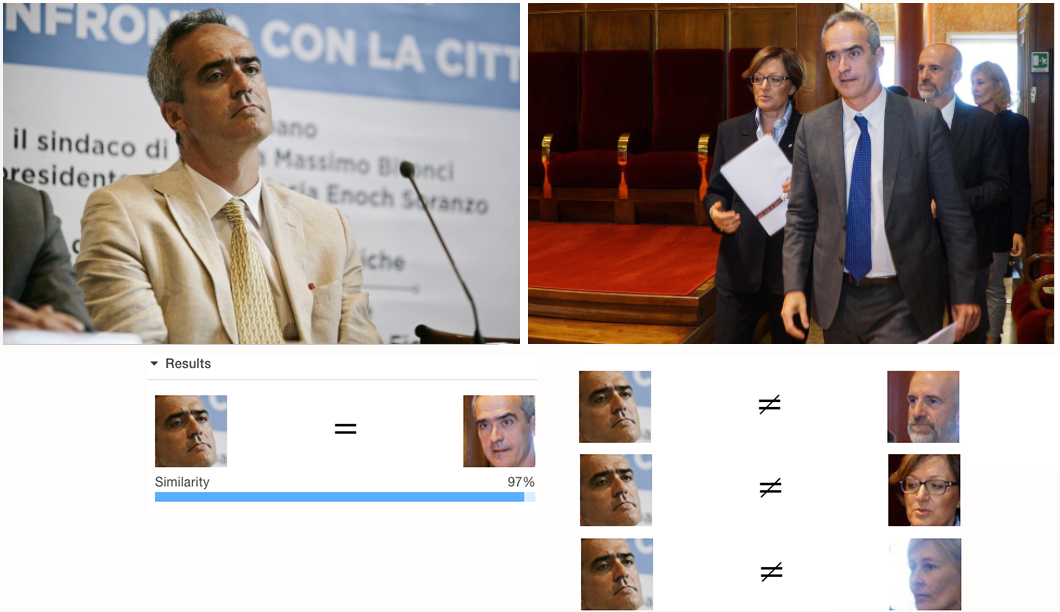
\includegraphics[width=.8\textwidth,keepaspectratio=true]{esempi-amazon/confronto}
		\label{fig:esempio-amazon}
	\end{figure}
\end{frame}
%
%----------------------------------------------------------------------------------------
%	APPUNTI:
% 		-
%----------------------------------------------------------------------------------------


	%----------------------------------------------------------------------------------------
	%	GOOGLE - 0
	%----------------------------------------------------------------------------------------
	% !TEX encoding = UTF-8
% !TEX program = pdflatex
% !TEX root = presentazione.tex
% !TeX spellcheck = it_IT
%
\begin{frame}[t]{Google Cloud Machine Learning Servicess}
	\begin{figure}[!h]
	\centering
	\vfill
	
\includegraphics[width=.3\paperwidth,keepaspectratio=true]{loghi/google-cp}
	\vfill
	\end{figure}
\end{frame}
%
%----------------------------------------------------------------------------------------
%	APPUNTI:
%		-
%----------------------------------------------------------------------------------------


	%----------------------------------------------------------------------------------------
	%	GOOGLE
	%----------------------------------------------------------------------------------------
	% !TEX encoding = UTF-8
% !TEX program = pdflatex
% !TEX root = presentazione.tex
% !TeX spellcheck = it_IT
%
\begin{frame}[t]{Google Cloud Vision API}
\begin{itemize}
	\item Rilevamento:
	\begin{itemize}
		\item oggetti e scene
		\item volti
		\item testo
		\item luoghi d'interesse
		\item loghi
		\item contenuti non adatti ai minori
	\end{itemize}
	\item Entità Web
\end{itemize}
\end{frame}
%
%----------------------------------------------------------------------------------------
%	APPUNTI:
% 		- testo: sia normale (lettere -> parole -> frasi) che su immagini con molto testo
%		- luoghi interesse: famosi elementi naturali e artificiali
%		- web detection:
%			- webEntities: deduce elementi dell’immagine da immagini simili nel web
%			- fullMatchingImages: immagini presenti nel web molto simili a quella di partenza
%			- partialMatchingImages
%			- pagesWithMatchingImages pagine web che contengono imm. simili a quella di partenza
%----------------------------------------------------------------------------------------


	%----------------------------------------------------------------------------------------
	%	SLIDE 17: GOOGLE - 2
	%----------------------------------------------------------------------------------------
	% !TEX encoding = UTF-8
% !TEX program = pdflatex
% !TEX root = presentazione.tex
% !TeX spellcheck = it_IT
%
\begin{frame}[t]{Google Cloud Vision API - Esempio}
	\begin{figure}[h]
	\centering
	    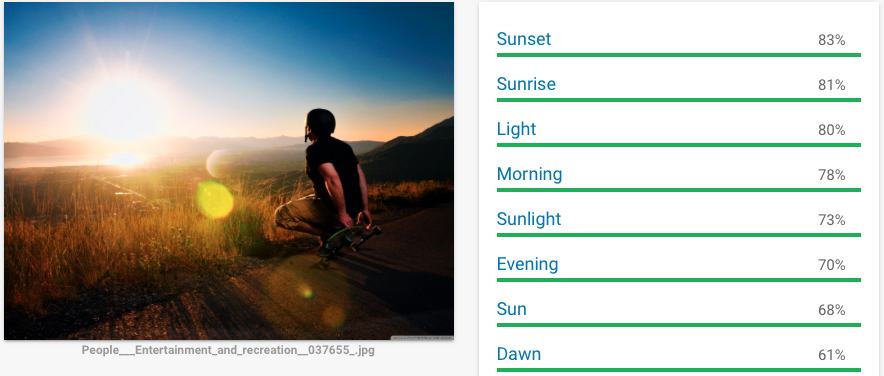
\includegraphics[width=\textwidth,keepaspectratio=true]{esempi-google/tagging}
		\label{fig:esempio-google}
	\end{figure}
\end{frame}
%
%----------------------------------------------------------------------------------------
%	APPUNTI:
% 		-
%----------------------------------------------------------------------------------------


	%----------------------------------------------------------------------------------------
	%	GOOGLE - 3
	%----------------------------------------------------------------------------------------
	% !TEX encoding = UTF-8
% !TEX program = pdflatex
% !TEX root = presentazione.tex
% !TeX spellcheck = it_IT
%
\begin{frame}[t]{Google Cloud Vision API - Esempio (2)}
	\begin{figure}[h]
	\centering
	    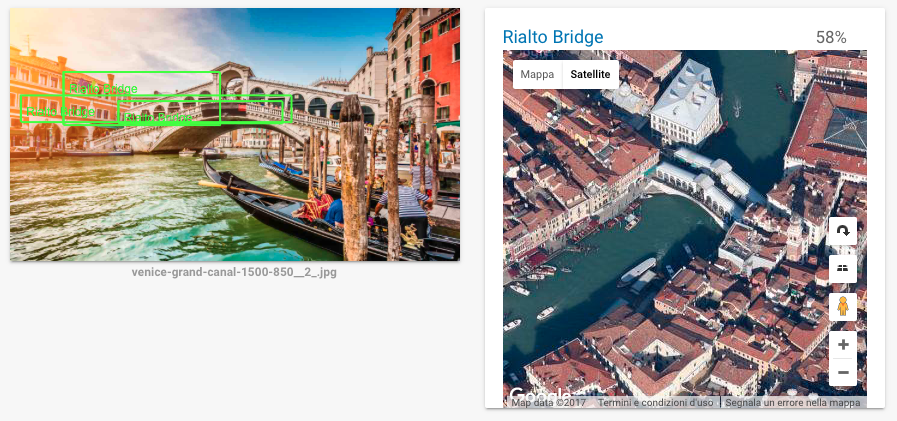
\includegraphics[width=\textwidth,keepaspectratio=true]{esempi-google/landmark}
		\label{fig:esempio-google-2}
	\end{figure}
\end{frame}
%
%----------------------------------------------------------------------------------------
%	APPUNTI:
% 		-
%----------------------------------------------------------------------------------------


	%----------------------------------------------------------------------------------------
	%	GOOGLE - 4
	%----------------------------------------------------------------------------------------
	% !TEX encoding = UTF-8
% !TEX program = pdflatex
% !TEX root = presentazione.tex
% !TeX spellcheck = it_IT
%
\begin{frame}[t]{Google Cloud Vision API - Esempio (3)}
	\begin{figure}[h]
	\centering
	    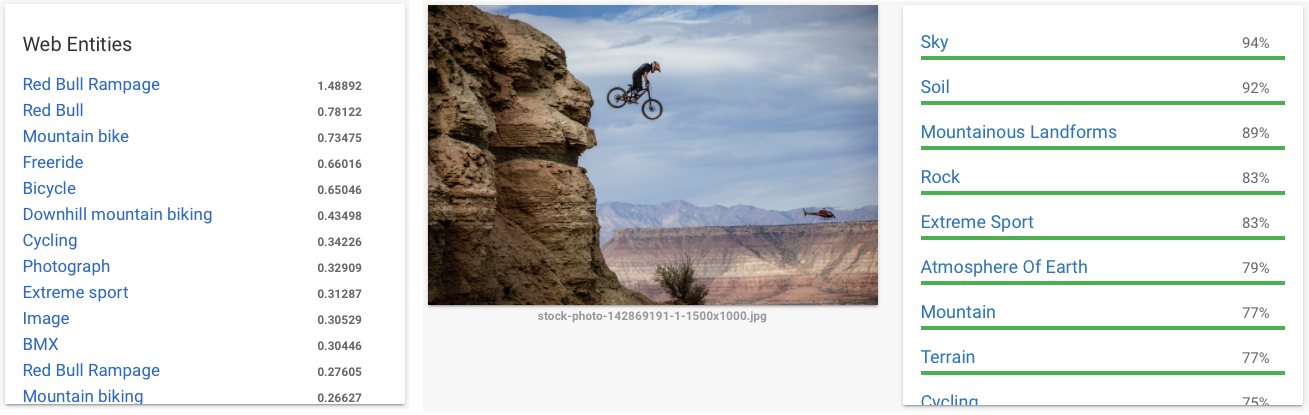
\includegraphics[width=\textwidth,keepaspectratio=true]{esempi-google/web}
		\label{fig:esempio-google-3}
	\end{figure}
\end{frame}
%
%----------------------------------------------------------------------------------------
%	APPUNTI:
% 		- score: Overall relevancy score for the entity. Not normalized and not comparable across different image queries.
%----------------------------------------------------------------------------------------


	%----------------------------------------------------------------------------------------
	%	CONFRONTO - 1
	%----------------------------------------------------------------------------------------
	% !TEX encoding = UTF-8
% !TEX program = pdflatex
% !TEX root = presentazione.tex
% !TeX spellcheck = it_IT
%
\begin{frame}[t]{Servizi a confronto - Riconoscimento oggetti}
	\begin{figure}[h]
	\centering
		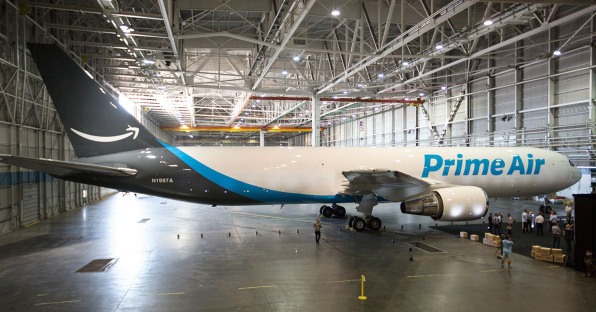
\includegraphics[width=.9\textwidth,keepaspectratio=true]{../../doc/img/prime-air}
		\label{fig:confronto-prime-air}
	\end{figure}
\end{frame}
%
%----------------------------------------------------------------------------------------
%	APPUNTI:
% 		-
%----------------------------------------------------------------------------------------


	%----------------------------------------------------------------------------------------
	%	CONFRONTO - 2
	%----------------------------------------------------------------------------------------
	% !TEX encoding = UTF-8
% !TEX program = pdflatex
% !TEX root = presentazione.tex
% !TeX spellcheck = it_IT
%
\begin{frame}[t]{Servizi a confronto - Riconoscimento oggetti}
	\begin{table}[!h]
		\centering
		{\tiny
		\resizebox{.9\paperwidth}{!}{
		\begin{tabularx}{\paperwidth}{l?l|l|l|l}
		\toprule
								& Microsoft C.S   & IBM W.S.       & Amazon A. I. & Google C.M.L.S. \\ \hline
		\midrule
		Etichette   			& plane (97,41\%)                & hangar (97,9\%)           & Hangar (95,74\%)               & Airliner (96\%)             \\
		& indoor (96,20\%)               & blue color (85,9\%)       & Aircraft (89,96\%)             & Airline (95\%)              \\
		& floor (96,10\%)                & steel blue color (75,5\%) & Airplane (89,96\%)             & Airplane (95\%)             \\
		& airplane (91,19\%)             &                           & Warplane (66,30\%)             & Vehicle (91\%)              \\
		& airport (91,11\%)              &                           & Jet (57,09\%)                  & Air travel (90\%)           \\
		& aircraft (72,66\%)             &                           & Landing (52,80\%)              & Aircraft (87\%)             \\
		& transport (67,56\%)            &                           &                                & Aviation (85\%)              \\	\hline
		Descrizione & a large airplane at an airport & -                         & -                              & -				\\
		\bottomrule
		\end{tabularx}}
		{\tiny \caption{Tabella riassuntiva per il riconscimento oggetti e ambientazione.}}
		\label{tab:riconscimento-oggetti-ambientazione}}
	\end{table}
\end{frame}
%
%----------------------------------------------------------------------------------------
%	APPUNTI:
% 		-
%----------------------------------------------------------------------------------------


	%----------------------------------------------------------------------------------------
	%	CONFRONTO - 3
	%----------------------------------------------------------------------------------------
	% !TEX encoding = UTF-8
% !TEX program = pdflatex
% !TEX root = presentazione.tex
% !TeX spellcheck = it_IT
%
\begin{frame}[t]{Servizi a confronto - Riconoscimento volto}
	\begin{figure}[!h]
	\begin{center}
		\resizebox{.9\paperwidth}{!}{
		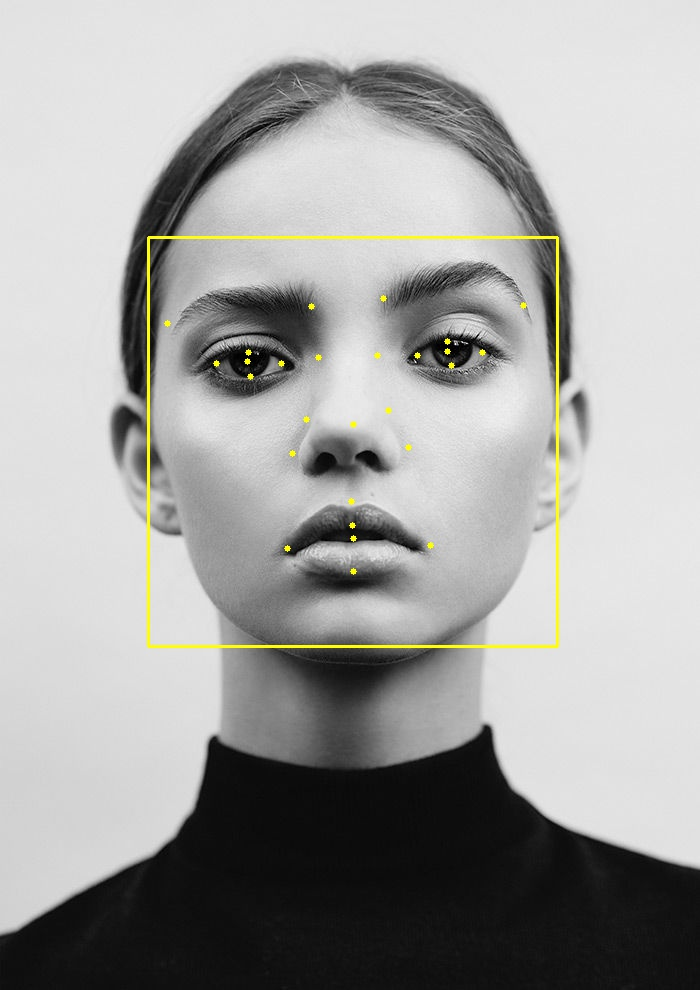
\includegraphics[width=200px,height=282px]{../../doc/img/riconoscimento-viso-1/microsoft.jpg}
		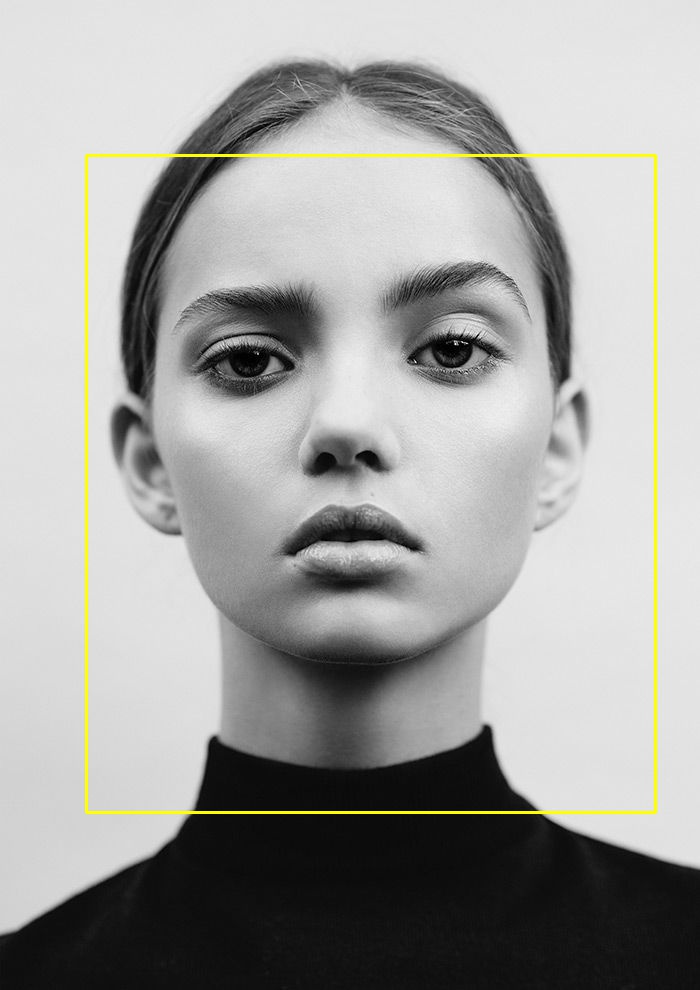
\includegraphics[width=200px,height=282px]{../../doc/img/riconoscimento-viso-1/ibm.jpg}
		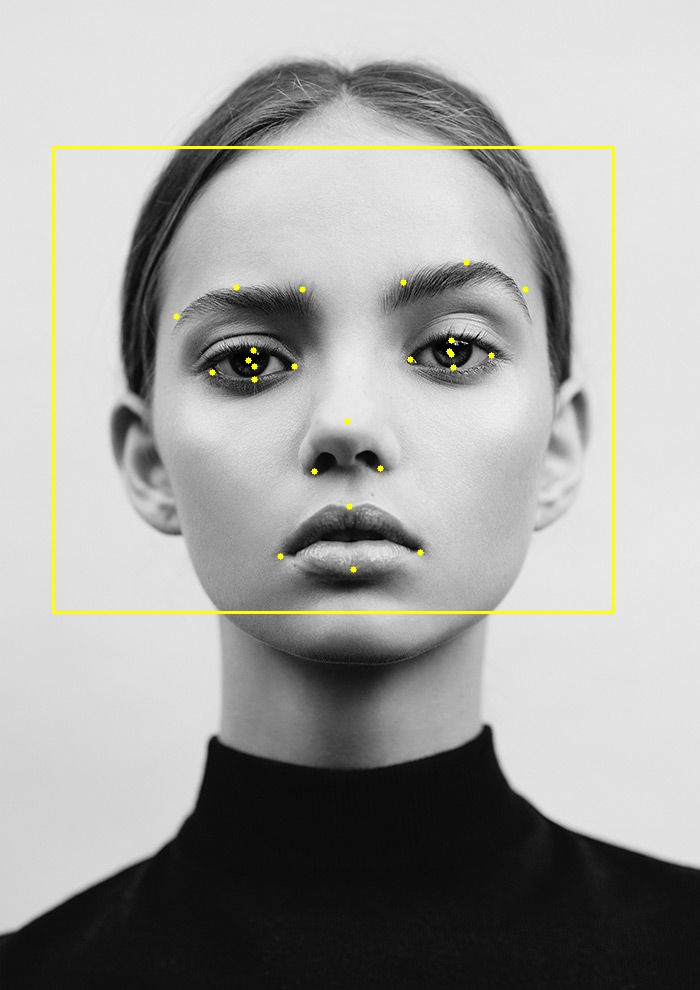
\includegraphics[width=200px,height=282px]{../../doc/img/riconoscimento-viso-1/amazon.jpg}
		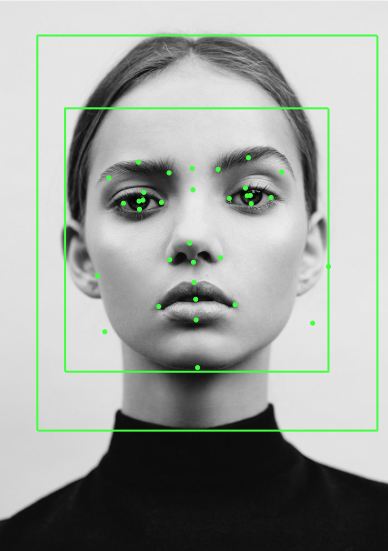
\includegraphics[width=200px,height=282px]{../../doc/img/riconoscimento-viso-1/google.png}
		}
	{\tiny \caption{Da sinistra: Microsoft, IBM, Amazon, Google.}
	\label{fig:riconscimento-volto-singolo}}
	\end{center}
	\end{figure}
\end{frame}
%
%----------------------------------------------------------------------------------------
%	APPUNTI:
% 		-
%----------------------------------------------------------------------------------------


	%----------------------------------------------------------------------------------------
	%	TARIFFE
	%----------------------------------------------------------------------------------------
	% !TEX encoding = UTF-8
% !TEX program = pdflatex
% !TEX root = presentazione.tex
% !TeX spellcheck = it_IT
%
\begin{frame}[t]{Tariffe - Microsoft Computer Vision API}
	\begin{itemize}
		\item Piano gratuito [chiamate all'API mensili]:
		\begin{itemize}
			\item 5000
			\item max 20 chiamate al minuto
		\end{itemize}
		\item Piani a pagamento:
		\begin{itemize}
			\item prezzo in base al metodo utilizzato e alla quantità
			\item Es. Tagging: 1\$ ogni 1000 chiamate/mese (fino a 1M)
		\end{itemize}
	\end{itemize}
\end{frame}
%
%----------------------------------------------------------------------------------------
%	APPUNTI:
%		- Face API limite a 30K al mese per il gratuito e mediamente costa un po' di piùs
%		- Computer Vision API - tagging: 0,8$ fino a 5M e 0,65$ fino a 20M
%		-
%----------------------------------------------------------------------------------------


	%----------------------------------------------------------------------------------------
	%	TARIFFE - 2
	%----------------------------------------------------------------------------------------
	% !TEX encoding = UTF-8
% !TEX program = pdflatex
% !TEX root = presentazione.tex
% !TeX spellcheck = it_IT
%
\begin{frame}[t]{Tariffe - IBM Visual Recognition}
\begin{itemize}
	\item Piano gratuito:
	\begin{itemize}
		\item 250 immagini al giorno
		\item un classificatore personalizzato con 5000 immagini
		\item della durata di 30 giorni.
	\end{itemize}
	\item Piano standard:
	\begin{itemize}
		\item 25000 chiamate al giorno
		\item classificazione: [singola chiamata all'API]
		\begin{itemize}
			\item standard: 0,002\$
			\item con classificatore personalizzato: 0,004\$
		\end{itemize}
		\item volti: 0,004\$ a chiamata
		\item addestramento classificatore: 0,10\$ a immagine
	\end{itemize}
\end{itemize}
\end{frame}
%
%----------------------------------------------------------------------------------------
%	APPUNTI:
%		- 250 al giorno = 7500 al mese (però conteggio giornaliero)
%----------------------------------------------------------------------------------------


	%----------------------------------------------------------------------------------------
	%	TARIFFE - 3
	%----------------------------------------------------------------------------------------
	% !TEX encoding = UTF-8
% !TEX program = pdflatex
% !TEX root = presentazione.tex
% !TeX spellcheck = it_IT
%
\begin{frame}[t]{Tariffe - Piani a pagamento}
\begin{itemize}
	\item Variano in base alla funzionalità richiesta.
	\item Esempi [costo ogni 1000 chiamate all'API]:
	\begin{itemize}
		\item Vision API - riconscimento oggetti: 1\$
		\item Vision API - descrizione: 1,5\$
		\item Visual Recognition: 2\$
		\item Reckognition: 1\$
		\item Cloud Vision - riconscimento oggetti: 1,5\$
		\item Cloud Vision - riconscimento Web: 3,5\$
	\end{itemize}
\end{itemize}
\end{frame}
%
%----------------------------------------------------------------------------------------
%	APPUNTI:
%		- costi per il primo milione al mese
%		- ibm fattura a immagine, non ogni 1000
%		- generlamente per i volti costa di più (soprattutto per IBM)
%----------------------------------------------------------------------------------------


	%----------------------------------------------------------------------------------------
	%	TARIFFE - 4
	%----------------------------------------------------------------------------------------
	% !TEX encoding = UTF-8
% !TEX program = pdflatex
% !TEX root = presentazione.tex
% !TeX spellcheck = it_IT
%
\begin{frame}[t]{Tariffe - Google Cloud Vision API}
\begin{itemize}
	\item Piano gratuito:
	\begin{itemize}
		\item 1000 chiamate al mese
	\end{itemize}
	\item Pianio a pagamento:
	\begin{itemize}
		\item varia in base al metodo utilizzato e al numero di chiamate
		\item Es. \textsf{Label Detection}: 1,50\$ ogni 1000 chiamate fino a 1M
		\item Es. \textsf{Web Detection}: 3,50\$ ogni 1000 chiamate fino a 1M
	\end{itemize}
\end{itemize}
\end{frame}
%
%----------------------------------------------------------------------------------------
%	APPUNTI:
%		- 1K-1M al mese
%----------------------------------------------------------------------------------------


	%----------------------------------------------------------------------------------------
	%	TARIFFE - 5
	%----------------------------------------------------------------------------------------
	% !TEX encoding = UTF-8
% !TEX program = pdflatex
% !TEX root = presentazione.tex
% !TeX spellcheck = it_IT
%
\begin{frame}[t]{Tariffe - Confronti}
	\begin{figure}[h]
	\centering
	    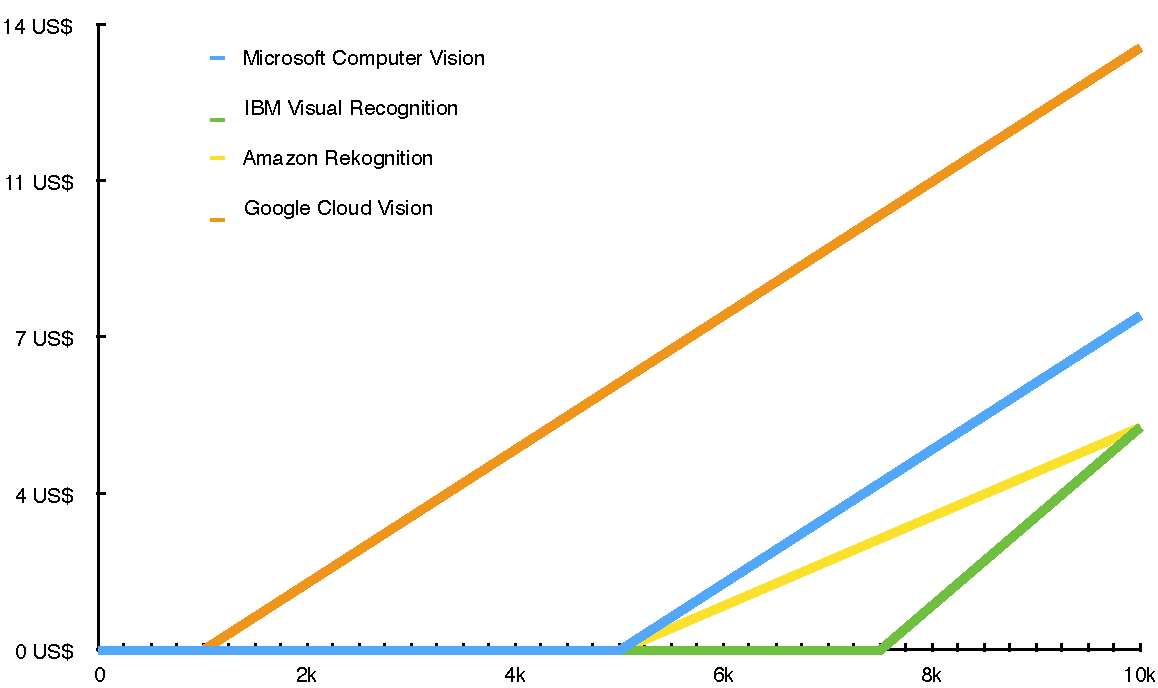
\includegraphics[width=.6\paperwidth,keepaspectratio=true]{../../doc/img/grafico1}
		{\tiny \caption{Riconoscimento oggetti con piano gratuito (da 0 a 10K immagini).}}
		\label{fig:tariffe-riconoscimento-oggetti-con-gratuito}
	\end{figure}
\end{frame}
%
%----------------------------------------------------------------------------------------
%	APPUNTI:
% 		- ricordarsi che ibm ne ha di più ma fa il conteggio giornaliero
%		- contiamo 1 chiamata - 1 immagine così viene più semplice
%----------------------------------------------------------------------------------------


	%----------------------------------------------------------------------------------------
	%	TARIFFE - 6
	%----------------------------------------------------------------------------------------
	% !TEX encoding = UTF-8
% !TEX program = pdflatex
% !TEX root = presentazione.tex
% !TeX spellcheck = it_IT
%
\begin{frame}[t]{Tariffe - Confronti (2)}
	\begin{figure}[h]
	\centering
	    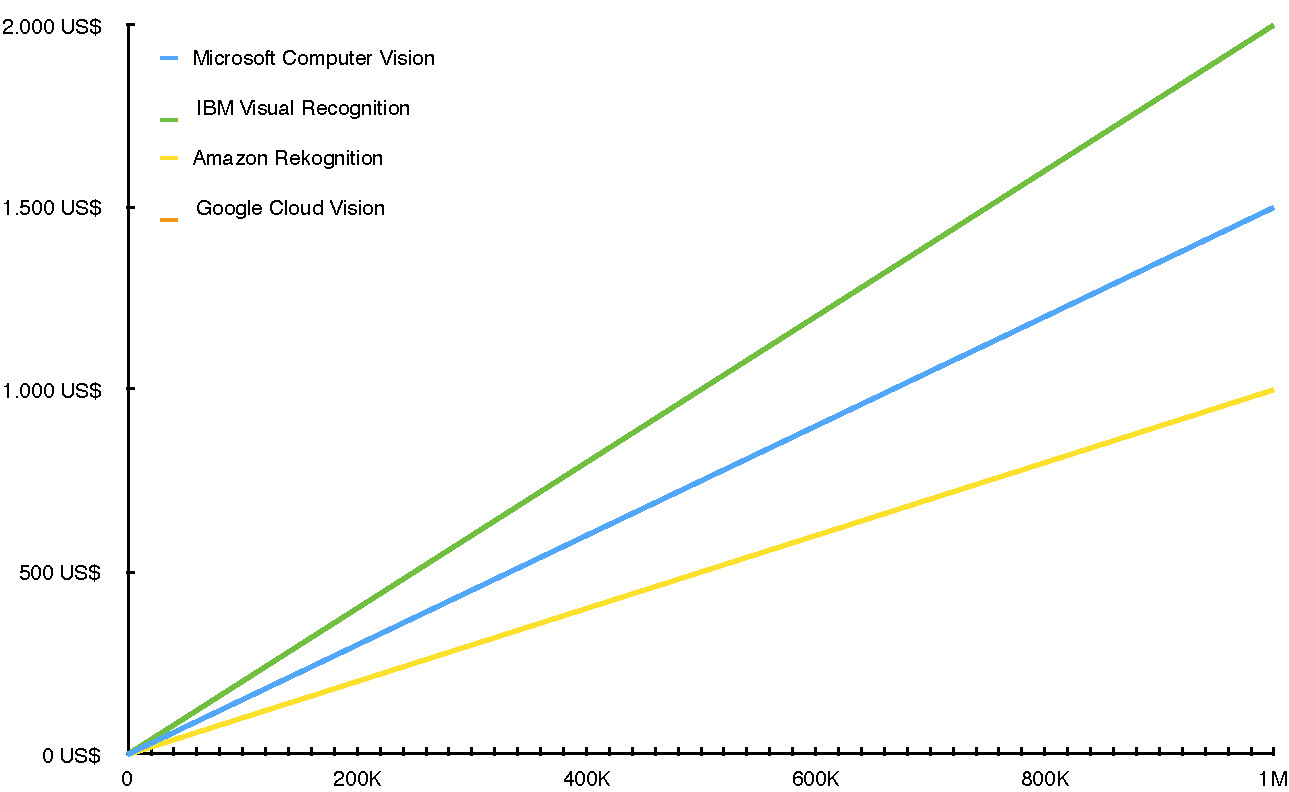
\includegraphics[width=.6\paperwidth,keepaspectratio=true]{../../doc/img/grafico2}
		{\tiny \caption{Riconoscimento oggetti senza piano gratuito (da 0 a 1M immagini).}}
		\label{fig:tariffe-riconoscimento-oggetti-senza-gratuito}
	\end{figure}
\end{frame}
%
%----------------------------------------------------------------------------------------
%	APPUNTI:
% 		-
%----------------------------------------------------------------------------------------


	%----------------------------------------------------------------------------------------
	%	TARIFFE - 7
	%----------------------------------------------------------------------------------------
	% !TEX encoding = UTF-8
% !TEX program = pdflatex
% !TEX root = presentazione.tex
% !TeX spellcheck = it_IT
%
\begin{frame}[t]{Tariffe - Confronti (3)}
	\begin{figure}[h]
	\centering
	    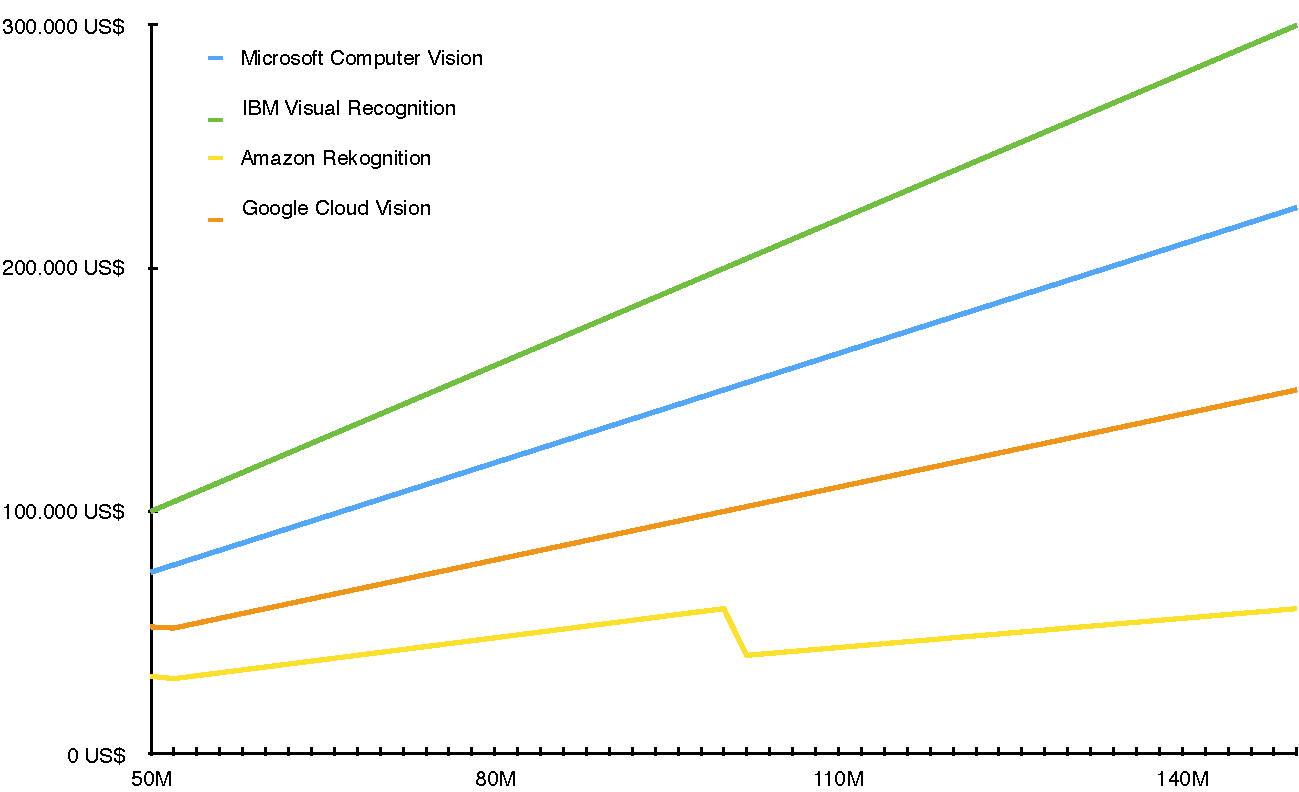
\includegraphics[width=.6\paperwidth,keepaspectratio=true]{../../doc/img/grafico3}
		{\tiny \caption{Riconoscimento oggetti (da 50M a 150M di immagini).}}
		\label{fig:tariffe-riconoscimento-oggetti-50-150M}
	\end{figure}
\end{frame}
%
%----------------------------------------------------------------------------------------
%	APPUNTI:
% 		- i prezzi sono proiezioni lineari di quelli base disponibili
%			per carichi così elevati probabilmente i prezzi si abbassano
%			- anche perché molti rendono disponibili prezzi fino a 20M altri fino a 1M
%		- TODO: sistemare: prima dicevo a chiamata, adessso uso a immagine.
%----------------------------------------------------------------------------------------


	%----------------------------------------------------------------------------------------
	%	CONCLUSIONI
	%----------------------------------------------------------------------------------------
	% !TEX encoding = UTF-8
% !TEX program = pdflatex
% !TEX root = presentazione.tex
% !TeX spellcheck = it_IT
%
\begin{frame}[t]{Conclusioni}
\begin{itemize}
	\item Le funzioni principali sono offerte da tutte le piattaforme
	\item Solo alcuni permettono la gestione di un classificatore
	\item Spesso le funzioni di ricerca/confronto sono limitate ai volti
	\item I risultati in risposta sono molto buoni
	\item Presenza di piani gratuiti
\end{itemize}
\end{frame}
%
%----------------------------------------------------------------------------------------
%	APPUNTI:
% 		-  I risultati in risposta sono molto buoni --> uno è meglio in una cosa,
%			l'altro in un'altra
%----------------------------------------------------------------------------------------


%----------------------------------------------------------------------------------------
%	FINE
%----------------------------------------------------------------------------------------
\section{Fine}\label{sec:fine}
% !TEX encoding = UTF-8
% !TEX program = pdflatex
% !TEX root = presentazione.tex
% !TeX spellcheck = it_IT
%
\nonumber
\begin{frame}[t,plain,noframenumbering]{Grazie per l'attenzione}
\begin{figure}[f]
\centering
	%\resizebox{.9\paperwidth}{.6\paperheight}{
	% Unipd logos
	\begin{columns}
		\begin{column}{0.5\paperwidth}
			\begin{figure}[!h]
			
\includegraphics[height=50px,keepaspectratio=true]{logo-unipd-int}
			\end{figure}
		\end{column}
		\begin{column}{0.5\textwidth}
			\begin{figure}[!h]
			
\includegraphics[width=120px,keepaspectratio=true]{logoDM}
			\end{figure}
		\end{column}
	\end{columns}
	\vspace{10px}
	% Services logos
	\begin{columns}
		\begin{column}{0.5\paperwidth}
			\begin{figure}[!h]
				
\includegraphics[height=35px,keepaspectratio=true]{loghi/microsoft-azure}
				\vfill
				\vspace{20px}
				
\includegraphics[height=60px,keepaspectratio=true]{loghi/ibm-bluemix}
			\end{figure}
		\end{column}
		\begin{column}{0.5\textwidth}
			\begin{figure}[!h]
				
\includegraphics[height=35px,keepaspectratio=true]{loghi/amazon-ws}
				\vfill
				\vspace{20px}
				
\includegraphics[height=50px,keepaspectratio=true]{loghi/google-cp}
			\end{figure}
		\end{column}
	\end{columns}
	%}
\end{figure}
\end{frame}
%
%----------------------------------------------------------------------------------------
%	APPUNTI:
% 		-
%----------------------------------------------------------------------------------------


%----------------------------------------------------------------------------------------
%	APPENDICI
%----------------------------------------------------------------------------------------
%\appendix


	%----------------------------------------------------------------------------------------
	%	END
	%----------------------------------------------------------------------------------------

\end{document}
